\documentclass{article}
\usepackage{../repsty}

\usepackage[standard,amsmath,thmmarks,hyperref,thref]{ntheorem}	

\theoremseparator{.}
\theorembodyfont{\normalfont}
\theoremsymbol{\ensuremath{\qed}}
\renewtheorem{Definition}{Def.}

\newcommand{\err}{\epsilon}

\DeclareDocumentCommand{\CS}{sO{}}{\IfBooleanTF{#1}{\hat{\sigma}_{#2}}{\sigma_{#2}}}
\DeclareDocumentCommand{\slp}{sO{}}{\IfBooleanTF{#1}{\hat{\beta}_{#2}}{\beta_{#2}}}
\DeclareDocumentCommand{\Thick}{O{}}{\Theta_{#1}}

\DeclareDocumentCommand{\SE}{sm}{\IfBooleanTF{#1}{\hat{\sigma}\bkt*{#2}}{\sigma\bkt*{#2}}}

\DeclareDocumentCommand{\bkt}{sm}{\IfBooleanTF{#1}{\left[ #2 \right]}{\left(#2\right)}}
\newcommand{\td}{\mathrm{d}}

\DeclareDocumentCommand{\Ayy}{sO{}}{\IfBooleanTF{#1}{\hat{A}_{y,y}}{A_{y,y}}^{#2}}
\DeclareDocumentCommand{\D}{s}{\IfBooleanTF{#1}{\hat{D}}{D}}
\DeclareDocumentCommand{\R}{s}{\IfBooleanTF{#1}{\hat{R}}{R}}
\DeclareDocumentCommand{\DP}{s}{\IfBooleanTF{#1}{(P^+ - P^-)}{\Delta P}}
\DeclareDocumentCommand{\SP}{s}{\IfBooleanTF{#1}{(P^+ + P^-)}{\Sigma P}}

\begin{document}

\section{$\Ayy$ estimators}

Assuming the model for the slope of $\ln I_t = \ln I_0 + \slp t + \err_t + \CS[0]$ is 
\begin{align*}
\slp &= -\nu\CS[X]\Thick[X] - \nu\CS[0]\Thick\bkt{1 + PP^t \Ayy} \\
	 &= - \nu\CS[0]\Thick\bkt{1 + x + PP^t \Ayy},\\ 
x 	 &= \frac{\CS[X]\Thick[X]}{\CS[0]\Thick},
\end{align*}
two ways to construct the estimator for $\Ayy$ are via the slope difference $\D = \slp^- - \slp^+ = \nu\CS[0]\Thick P^t \DP* \Ayy$, with the corresponding \emph{difference} estimator 
\[
	\Ayy*[D] = \bkt{\nu\CS[0]\Thick}^{-1}\cdot\frac{\D*}{P^t\DP},
\]
or the slope ratio $\delta = \slp^+/\slp^-$, and the R-statistic
\[
	\R = \frac{\delta - 1}{\delta + 1} = \frac{\DP* P^t\Ayy}{2\cdot\bkt{1 + x} + \SP* P^t\Ayy},
\]
with the \emph{ratio} estimator
\[
	\Ayy*[R] = \frac{2\R*}{P^t\bkt{\DP -\R*\cdot\SP}}\cdot\bkt{1+x}.
\]

\section{Comparison of the estimators}

\subsection{Estimation of the asymmetry}
The compution of the asymmetry from the difference statistic requires knowledge of the product $\CS[0]\Thick$. The non-target scattering term $x$ could take any (unknown) value, however, so long as it is fixed and its variance satisfies statistical precision requirements. This cannot be said of the ratio estimator, in which $x$ remains as a nuisance parameter. 

The trade-off between the two estimators, therefore, is: if the value of $\CS[0]\Thick$ is known to a reasonable precision, the difference estimator trupms the ratio one; if, however, there's no way to know $\CS[0]\Thick$ itself reasonably well, it might be easier to estimate the ratio $\sfrac{\CS[X]\Thick[X]}{\CS[0]\Thick}$. 

It must be said, though, that systematic varying of $x$, causing grief to both estimators, causes \emph{more} to the R one. Compare:
\begin{align*}
\Ayy*[D] &= \frac{\D*}{\nu\CS[0]\Thick P^t\DP} - \frac{\Delta x}{P^t\DP},
\shortintertext{versus}
\Ayy*[R] &= \frac{\bkt{2+\Sigma x} \R*}{P^t\bkt{\DP-\R*\SP}} - \frac{\Delta x}{P^t\bkt{\DP-R\SP}}.
\end{align*}

\subsection{Systematic effects}
We could try to learn \emph{something} about the structure of the experiment by comparing the R- and D-statistics.
\DeclareDocumentCommand{\g}{s}{\IfBooleanT{#1}{\hat}g}

If we plot the QQ-plot of $\R*' \equiv \sfrac{2\R*}{P^t\bkt{\DP - \R*\SP}}$ against $\D*$, Fig.~\ref{fig:QQPlot_DR}, we see that the statistics' distributions are linearly related (the points of the QQ-plot lie on a line).
\begin{figure}[h]
\centering
\begin{subfigure}{.5\textwidth}
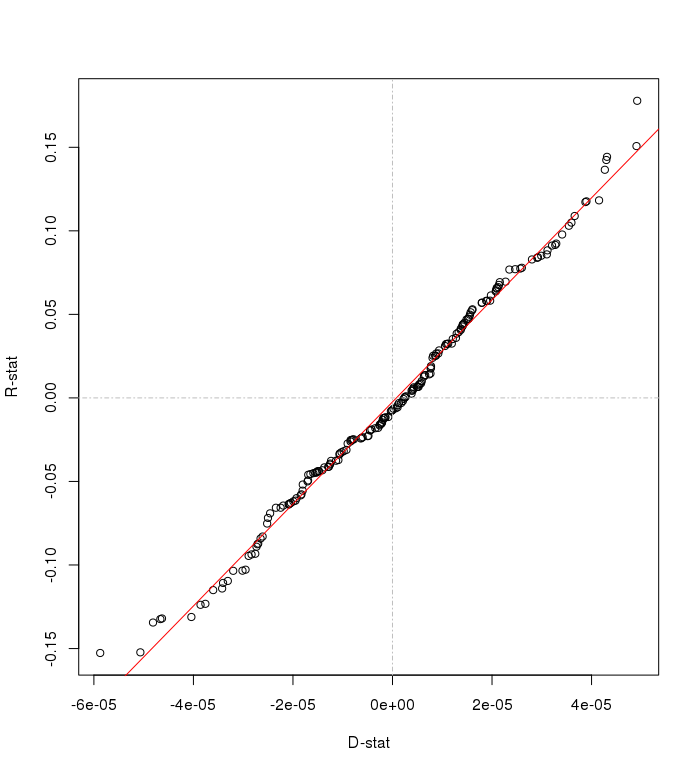
\includegraphics[scale=.5]{R_D_QQPlot}
\caption{Red line $y = a + b\cdot x$.}
\end{subfigure}~
\begin{subfigure}{.5\textwidth}
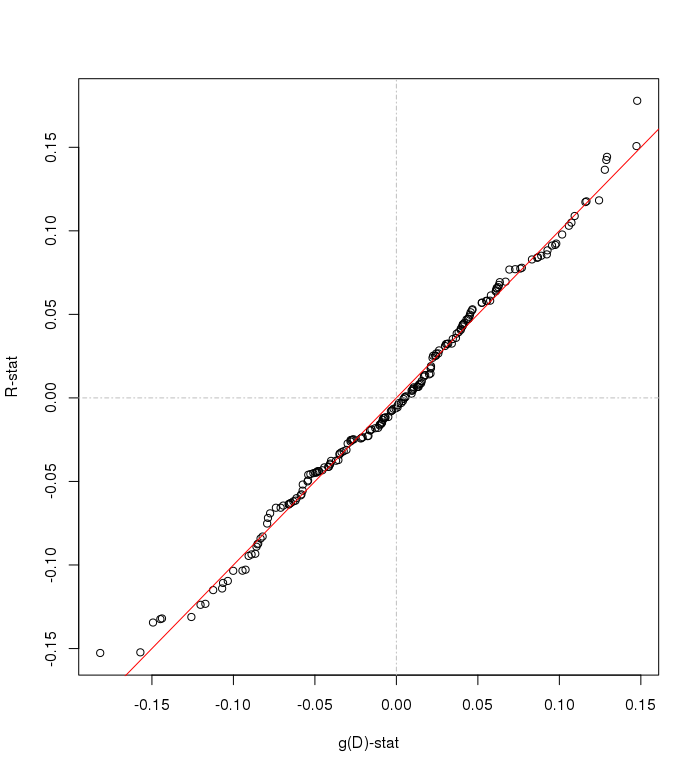
\includegraphics[scale=.5]{R_gD_QQPlot}
\caption{Red line $y = x$.}
\end{subfigure}
\caption{QQ-Plot for the sample quantiles of the R vs D statistics.\label{fig:QQPlot_DR}}
\end{figure}

By fitting this plot, we can find the linear transformation \emph{for the given sample} of slopes $\g*(\D*) = \hat\alpha + \hat\beta\D* = \sfrac{2\R*}{P^t\bkt{\DP - \R*\SP}}$

This means that
\begin{equation*}
\begin{cases}
	\Ayy*[R] &= \g*(\D*)\cdot(1+x), \\
	\D* 	 &= \Ayy*[D]\cdot\bkt{P^t\DP\nu\CS[0]\Thick};
\end{cases}
\end{equation*}
hence
\[
	\Ayy*[R] = (1+x) \cdot \bkt*{\hat\alpha + \hat\beta\cdot\bkt{P^t\DP\nu\CS[0]\Thick}\cdot\Ayy*[D]}
\]

%\section{Estimation of $x$}
%
%Assume the following model:
%\begin{equation*}
%\begin{cases}
%	\slp[0] &= -\nu\CS[X]\Thick[X], \\
%	\slp[1] &= -\nu\CS[X]\Thick[X] - \nu\CS[0]\Thick\bkt{1 + PP^t\Ayy}.
%\end{cases}
%\end{equation*}
%
%Then, we can write the model $\slp[1] = \alpha + \beta\slp[0] + \err$, where $\beta$ should be 



\end{document}